% ------------------------------------------------------------------------
% ------------------------------------------------------------------------
% abnTeX2: Modelo de Trabalho Academico (tese de doutorado, dissertacao de
% mestrado e trabalhos monograficos em geral) em conformidade com 
% ABNT NBR 14724:2011: Informacao e documentacao - Trabalhos academicos -
% Apresentacao
% ------------------------------------------------------------------------
% ------------------------------------------------------------------------

\documentclass[
	% -- opções da classe memoir --
	11pt,				% tamanho da fonte
	openany,			% capítulos começam em pág ímpar (insere página vazia caso preciso)
	oneside,
	%twoside,			% para impressão em verso e anverso. Oposto a oneside
	a4paper,			% tamanho do papel. 
	% -- opções da classe abntex2 --
	chapter=TITLE,		% títulos de capítulos convertidos em letras maiúsculas
	section=TITLE,		% títulos de seções convertidos em letras maiúsculas
	%subsection=TITLE,	% títulos de subseções convertidos em letras maiúsculas
	%subsubsection=TITLE,% títulos de subsubseções convertidos em letras maiúsculas
	% -- opções do pacote babel --
	english,			% idioma adicional para hifenização
	%french,				% idioma adicional para hifenização
	%spanish,			% idioma adicional para hifenização
	brazil				% o último idioma é o principal do documento
	]{abntex2}

% ---
% Pacotes
% ---

%\documentclass{report}
\usepackage{graphicx}
\usepackage{config}
\usepackage{caption}
\usepackage{lmodern}			% Usa a fonte Latin Modern			
\usepackage[T1]{fontenc}		% Selecao de codigos de fonte.
\usepackage[utf8]{inputenc}		
\usepackage{lastpage}			% Usado pela Ficha catalográfica
\usepackage{indentfirst}		% Indenta o primeiro parágrafo de cada seção.
\usepackage{color}				% Controle das cores
\usepackage{graphicx}			% Inclusão de gráficos
\usepackage{microtype} 			% para melhorias de justificação
\usepackage{lipsum}				% para geração de dummy text
\usepackage[brazilian,hyperpageref]{backref}	 % Paginas com as citações na bibl
\usepackage[alf]{abntex2cite}	% Citações padrão ABNT
% ---
% Configurações do pacote backref
% Usado sem a opção hyperpageref de backref
\renewcommand{\backrefpagesname}{Citado na(s) página(s):~}
% Texto padrão antes do número das páginas
\renewcommand{\backref}{}
% Define os textos da citação
\renewcommand*{\backrefalt}[4]{
	\ifcase #1 %
		Nenhuma citação no texto.%
	\or
		Citado na página #2.%
	\else
		Citado #1 vezes nas páginas #2.%
	\fi}%
% ---

% ---
% Informações de dados para CABEÇALHO
% ---
\titulo{DESENVOLVIMENTO DO CIRCUITO DIGITAL DE UMA MÁQUINA DE CAFÉ}
% TODO: lista com vários autores
\autor{Douglas Oliveira de Jesus}
\local{Feira de Santana}
\data{2023}
% TODO: mudar para tutor
\tutor{Armando Sanca Sanca}
\modulo{TEC498 Projeto de Circuitos Digitais}
\instituicao{%
  \textbf{Universidade Estadual de Feira de Santana}
}
\departamento{Tecnologia}
  
\tipotrabalho{PROTÓTIPO DE UM PAINEL ELETRÔNICO DIGITAL}
% ---

% ---
% Configurações de aparência do PDF final

% alterando o aspecto da cor azul
\definecolor{blue}{RGB}{41,5,195}

% informações do PDF
\makeatletter
\hypersetup{
     	%pagebackref=true,
		pdftitle={\@title}, 
		pdfauthor={\@author},
    	pdfsubject={\imprimirpreambulo},
	    pdfcreator={LaTeX with abnTeX2},
		pdfkeywords={abnt}{latex}{abntex}{abntex2}{trabalho acadêmico}, 
		colorlinks=true,       		% false: boxed links; true: colored links
    	linkcolor=blue,          	% color of internal links
    	citecolor=blue,        		% color of links to bibliography
    	filecolor=magenta,      		% color of file links
		urlcolor=blue,
		bookmarksdepth=4
}
\makeatother
% --- 

% --- 
% Espaçamentos entre linhas e parágrafos 
% --- 

% O tamanho do parágrafo é dado por:
\setlength{\parindent}{1.3cm}

% Controle do espaçamento entre um parágrafo e outro:
\setlength{\parskip}{0.2cm}  % tente também \onelineskip
     
% ---
% compila o indice
% ---
\makeindex
% ---

% ----
% Início do documento
% ----
\begin{document}


\frenchspacing 
\textual
\pagestyle{uefs-pbl}
\aliaspagestyle{chapter}{uefs-pbl-capitulo}
\imprimircabecalho
\begingroup
\let\clearpage\relax
% -----------------------------------------------------------
% Resumo
\begin{resumoumacoluna}
\textit{Este relatório técnico descreve os seguintes passos para o desenvolvimento do circuito digital de uma máquina de café: desenho do diagrama de transição de estados, bem como sua tabela e minimização dos estados; codificação; escolha dos elementos de memória; tabela de excitação; equações de exitação e de saída e desenho do circuito. A produção foi solicitada pela disciplina de M.I de Circuitos Digitais, do curso de Engenharia de Computação da Universidade Estadual de Feira de Santana, utilizando a metodologia PBL (Problem Based Learning).}


 \vspace{\onelineskip}
 
 \noindent
 \textbf{Palavras-chaves}: Máquina de Estados, MEF, Circuitos Digitais.
\end{resumoumacoluna}
% ----------------------------------------------------------
%IMPORTAÇÂO DOS TÒPICOS
% ----------------------------------------------------------
\chapter{INTRODUÇÃO}

A indústria do café é um dos setores mais importantes e lucrativos do mercado de bebidas. Com a crescente demanda por café em todo o mundo e seguindo o problema fictício proposto pela disciplina do Módulo Integrador de Circuitos Digitais com base na metodologia PBL, a empresa MANDACARU SA identificou uma oportunidade de negócio e decidiu investir no desenvolvimento de Vending Machines para atender aos amantes da bebida durante seus "coffee breaks" em ambientes de trabalho.

Nesse contexto, a MANDACARU SA já desenvolveu um protótipo de hardware para a Coffee Machine, que consiste em um compartimento de água, um compartimento para as cápsulas, um compartimento para copos, botões de seleção dos produtos, um dispensador, uma bomba de pressurização e um circuito elétrico de aquecimento por indução. No entanto, para automatizar o processo de vendas, é necessário implementar um circuito digital capaz de reconhecer e validar as moedas inseridas pelos usuários.

O objetivo deste relatório técnico é apresentar uma proposta de construção lógica dos circuitos internos da Coffee Machine, utilizando máquinas de estados, a fim de garantir o correto funcionamento do sistema de vendas. Serão abordadas as principais características do protótipo, como os sensores de nível mínimo no compartimento de água e os sensores de presença nos compartimentos de cápsulas e de recepção de copos. Além disso, serão discutidos os requisitos específicos que o circuito digital deve atender, como a validação das moedas de acordo com os preços dos produtos, a exibição de mensagens de erro e a correta sequência de acionamento dos circuitos internos.

Para atingir esse objetivo, serão realizadas atividades como a análise detalhada dos requisitos do sistema, o projeto da lógica de funcionamento utilizando máquinas de estados, a seleção dos componentes eletrônicos adequados e a implementação do circuito digital. Serão consideradas também as diretrizes estabelecidas, como a exibição de informações relevantes no display da máquina, a utilização de LEDs para representar as saídas do sistema e a correta identificação e tratamento de situações de erro.

Ao final deste relatório, espera-se apresentar uma solução técnica eficiente e funcional para automatizar o processo de vendas da Coffee Machine, garantindo uma experiência satisfatória para os usuários e contribuindo para o sucesso do empreendimento da MANDACARU SA no mercado de café.

O projeto em questão requer a implementação de um circuito digital para a Coffee Machine, a fim de automatizar o processo de vendas através do reconhecimento de moedas. Dessa forma, será possível garantir a correta seleção e pagamento dos produtos disponíveis na máquina.

As funcionalidades essenciais que o circuito digital deve oferecer incluem a validação das moedas inseridas, verificando se correspondem aos valores dos produtos (café expresso, café com leite, chá de camomila e cappuccino), exibindo mensagens de erro caso seja detectada uma moeda inválida e devolvendo as cédulas ou moedas ao cliente. Além disso, o circuito deve monitorar os níveis mínimos de água, a presença de cápsulas e a disponibilidade de copos, exibindo mensagens de erro apropriadas caso algum desses elementos esteja em falta.

Para proporcionar uma interação clara e intuitiva com o usuário, a Coffee Machine deverá contar com um display que informe o produto escolhido, o valor total das cédulas inseridas e eventuais códigos de erro associados a ações incorretas. Os resultados das ações realizadas pelo circuito interno também serão representados por LEDs, que servirão como indicadores visuais das saídas do sistema.

É importante destacar que a máquina deve permanecer funcional mesmo em caso de situações adversas, evitando travamentos durante o processo de venda. Para isso, será necessário desenvolver uma lógica eficiente que permita a correta sequência de acionamento dos circuitos internos, ativando o aquecimento por indução 2 segundos após o início da pressurização de água, possibilitando a extração adequada do café e sua posterior disponibilização ao cliente pelo dispensador.


\include{textuais/referencialTeorico}

\chapter{METODOLOGIA}

\section{Recursos utilizados}
Em todo o processo de criação do protótipo , algumas ferramentas foram utilizadas como auxiliadoras no processo.

Para desenvolvimento das tabelas, foi utilizado a plataforma do Google Sheets, disponível virtualemnte. Para o desenho do circuito, o software Logisim foi utilizado como uma ferramenta poderosa de desenho e simulação. Na parte de registro, o Overleaf foi utilizado como uma ferramenta que permite escrever em LateX, utilizando o modelo da ABNT disponibilizado no site do Módulo Integrador de Circuitos Digitais da UEFS. O site foi escolhido por ter uma ótima estruturação de escrita e permitir o desenvolvimento em grupo dentro da plataforma. Além do Overleaf, também para registros, o Trello foi utilizado como uma tabela de registro do que foi tratado nas sessões armazenando as ideias, fatos, questões e metas propostos pela metodologia PBL. Os recursos bibliográficos estão apresentados na sessão de referência deste relatório.

\section{Escolha do modelo de máquina}

Máquinas de estados são modelos matemáticos amplamente utilizados na área de engenharia de sistemas digitais para descrever o comportamento sequencial de sistemas. Essas máquinas são compostas por um conjunto finito de estados, transições entre esses estados e ações associadas a essas transições. Elas desempenham um papel fundamental no projeto e implementação de circuitos lógicos que respondem a estímulos externos de forma controlada e previsível.

No contexto do projeto da Coffee Machine, a escolha do modelo de máquina de estados se baseia na necessidade de descrever o comportamento sequencial do sistema, que envolve desde a inserção e validação das moedas até a entrega do produto escolhido ao cliente. As máquinas de estados oferecem uma estrutura clara e organizada para especificar todas as etapas e condições necessárias para o funcionamento adequado do sistema.

A escolha do modelo de Mealy para a Coffee Machine tem como objetivo aproveitar a capacidade de considerar as entradas durante as transições de estados para otimizar o controle do sistema \cite{tocci2010sistemas}. Isso é particularmente relevante para o processo de validação das moedas, onde a decisão de aceitar ou rejeitar uma moeda depende tanto do estado atual quanto do valor inserido.

\section{Desenho do diagrama de transição de estados}

\begin{figure}[!h]
    \centering
    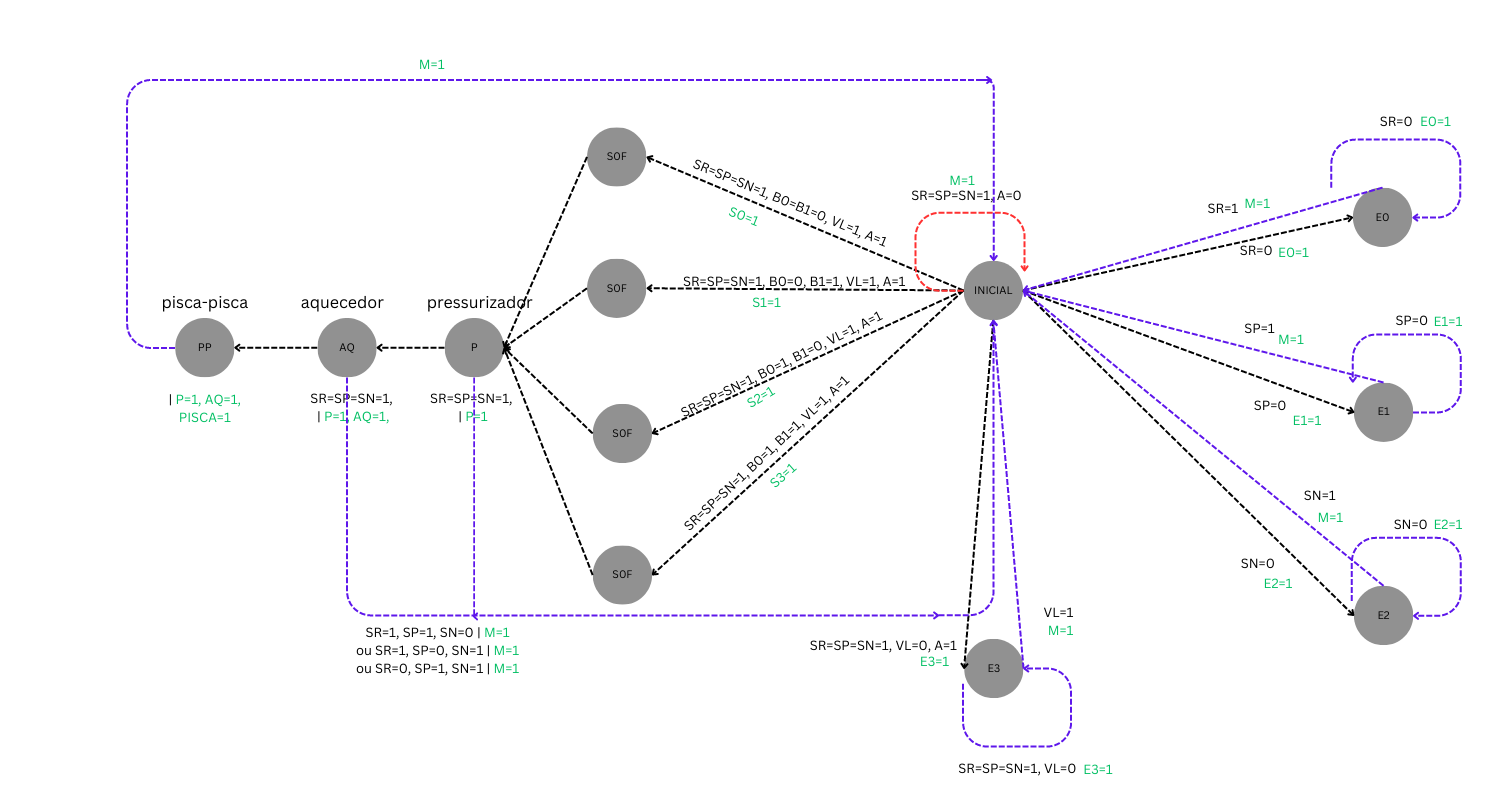
\includegraphics[width=1\textwidth]{imagens/diagramaDeTransicao.png}
    \caption{Desenho do diagrama de transição de estados}
    \label{fig:diagramaTransicao}
\end{figure}

No desenho do diagrama de transição de estados \ref{fig:diagramaTransicao}, o texto que descreve as entradas estão na cor preta e o texto que descreve as saídas estão na cor verde. As setas pretas seguem um fluxo a partir do estado inicial, enquanto as de outras cores voltam para o estado inicial, seja devido aos erros ou devido a finalização do processo. 

As saídas estão representadas pelos códigos:  E0, E1, E2, E3, S0, S1, S2, S3, P, AQ, PP. As saídas que irão acionar o display de led para demonstração de erros são: E0 (para o sensor SR), E1 (para o sensor SP), E2 (para o sensor SN) e E3 (valor não correspondente com bebida selecionada). Para o preparo da bebida: S0 (café expresso), S1 (café com leite), S2 (camomila) e S3 (cappuccino). Para representar o processo de preparo, seguem as seguintes saídas: P (pressurizador), AQ (aquecedor) e PP (pisca-pisca, que representa a liberação da bebida). Por fim, o M representa o modo de espera.

As entradas estão representadas pelos códigos: SR, SP, SN, A, VL (V0 e V1), B0, B1. As entradas dos sensores são o SR (copos), SP (cápsulas) e SN (nível mínimo). Para acionamento do pedido, há a entrada A. O VL entrará como um validador do valor selecionado. Se o valor selecionado (V0 e V1) estiver de acordo com a bebida selecionada (B0 e B1), VL será nível lógico alto (1). Caso contrário, será nível lógico baixo (0). Para efetuar a validação, as entradas V0 e V1 entraram no sistema, mas não entrarão na MEF, responsabilizando a entrada VL da MEF. Por fim, B0 e B1 são as entradas que representam a seleção da bebida. 

Os estados irão ter um atraso de transição de 2 segundos, para todas as exibições previstas a partir da saída serem efetuadas.

\section{Tabela de transição de estados e redução de estados}

Devido a máquina obter 7 entradas, 128 possibilidades são registradas apenas a partir do estado inicial. Tendo a noção que nem todas as possibilidades precisam ser registradas, já que várias entradas podem ser utilizadas como sem importância para as equações de excitação, a tabela foi definida de acordo com todas as possibilidades possíveis abstraídas. 

Os estados apresentados foram "INICIAL", que é o estado ideal de inicio da MEF, "EE0", "EE1", "EE2", "EE3", que representam os estados de erro dos sensores SR, SP, SN e da validação do valor e bebida, respectivamente, "ES0", "ES1", "ES2", "ES3", que representam a escolha da bebida com o valor inserido corretamente, "P" para presurização, "AQ" para aquecimento e "PP" para saída final, que será o acionamento contínuo de um LED. A Figura \ref{fig:tabelaTransicao} apresenta a tabela desenvolvida.

\begin{figure}[]
    \centering
    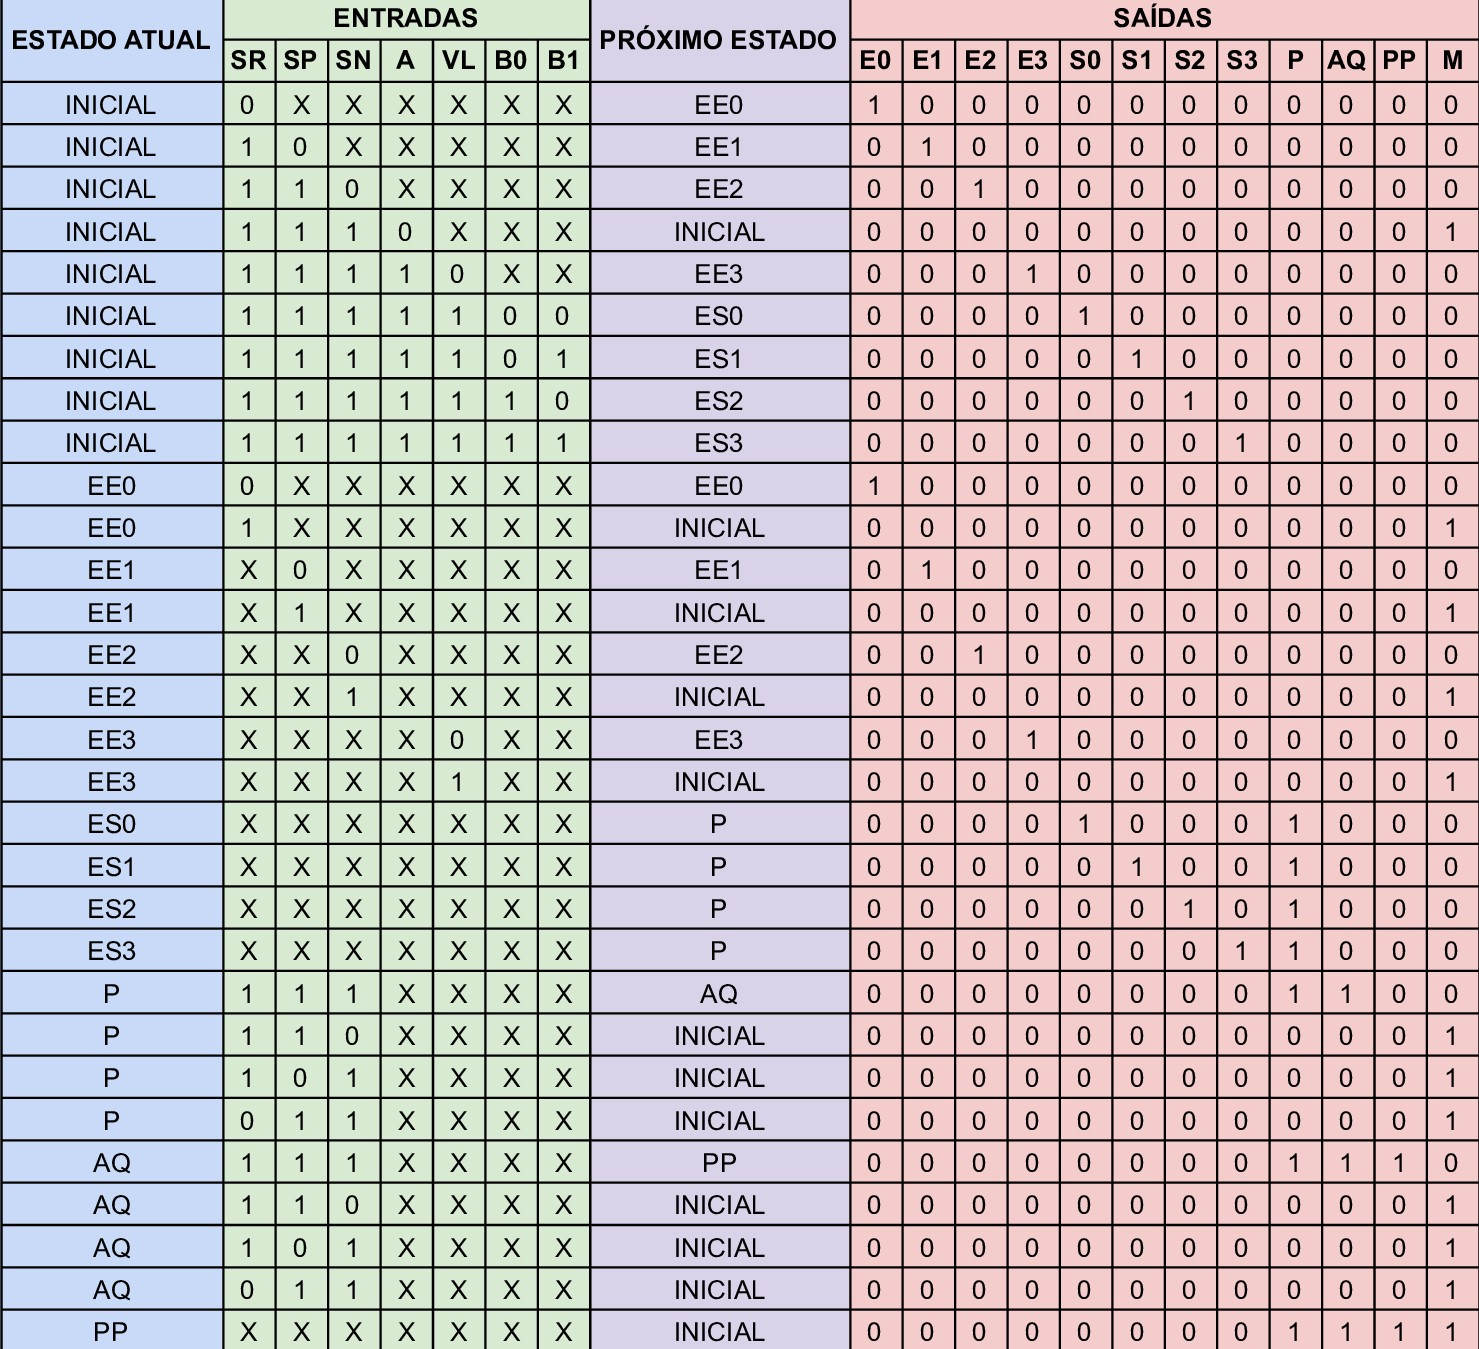
\includegraphics[width=1\textwidth]{imagens/tabelaDeTransicaoDeEstados.png}
    \caption{Tabela da transição de estados reduzida}
    \label{fig:tabelaTransicao}
\end{figure}

\section{Codificação de estados e modificação da tabela de transição de estados}

Como são 12 estados, serão necessários 4 flip-flops para construir a MEF, precisando de uma codificação de 4 bits. Foi decidido a seguinte representação:

\begin{itemize}
    \item INICIAL = 0000
    \item EE0 = 0001
    \item EE1 = 0010
    \item EE2 = 0011
    \item EE3 = 0100
    \item ES0 = 0101
    \item ES1 = 0110
    \item ES2 = 0111
    \item ES3 = 1000
    \item P = 1001
    \item AQ = 1010
    \item PP = 1011
\end{itemize}

A figura \ref{fig:tabelaCodificada} apresenta a codificação aplicada na tabela.

\begin{figure}[!h]
    \centering
    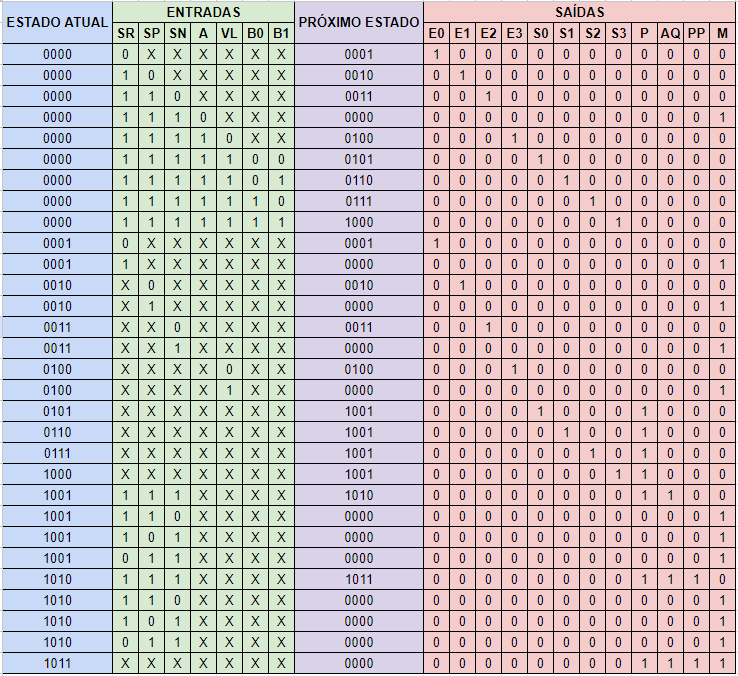
\includegraphics[width=1\textwidth]{imagens/tabelaCodificada.png}
    \caption{Tabela da transição de estados codificada}
    \label{fig:tabelaCodificada}
\end{figure}

\section{Escolha dos elementos de memória}

Para armazenar e representar os estados da máquina de estados, o flip-flop do tipo D é utilizado. Esse tipo de flip-flop possui uma entrada de dados (D) que determina o valor a ser armazenado e uma entrada de clock (CLK) que controla o momento de atualização do valor armazenado.

A escolha do flip-flop do tipo D se justifica pela sua simplicidade e facilidade de utilização, além de ser amplamente disponível e de baixo custo. Ele oferece a capacidade de armazenar e atualizar os estados da máquina de forma confiável e sincronizada com o clock do sistema \cite{floyd}.

Dessa forma, a combinação do modelo de máquina de estados de Mealy com o uso do flip-flop do tipo D proporciona uma abordagem adequada para o projeto da Coffee Machine. Essa escolha permite a especificação e implementação eficiente do controle do sistema, levando em consideração tanto o estado atual quanto as entradas relevantes para a geração de saída adequada.

\section{Construção da tabela e obtenção das equações de excitação}

Para gerar a tabela de excitação a partir de uma tabela codificada, é necessário tomar cada bit da quantidade de bits da codificação dos estados como a saída de um flip-flop. Como são 4 bits, serão 4 flip-flops. A expressão de saída pode ser construída através das situações onde a saída do flip-flop é 1. Para isso, basta registrar o estado atual de cada variável (saídas dos flip-flops atuais mais as entradas) através de min-terms. Uma forma de simplificar é utilizando o Mapa de Karnaugh, entretanto o mesmo não é recomendável para a quantidade de variáveis que são necessárias para cada termo da expressão da saída do flip-flop. Por isso, a simplificação será através da álgebra booleana. 

De acordo com a análise da Figura \ref{fig:tabelaExcitacao} é possível verificar quais são as expressões obtidas, utilizando a estratégia de min-terms.

\begin{figure}[!h]
    \centering
    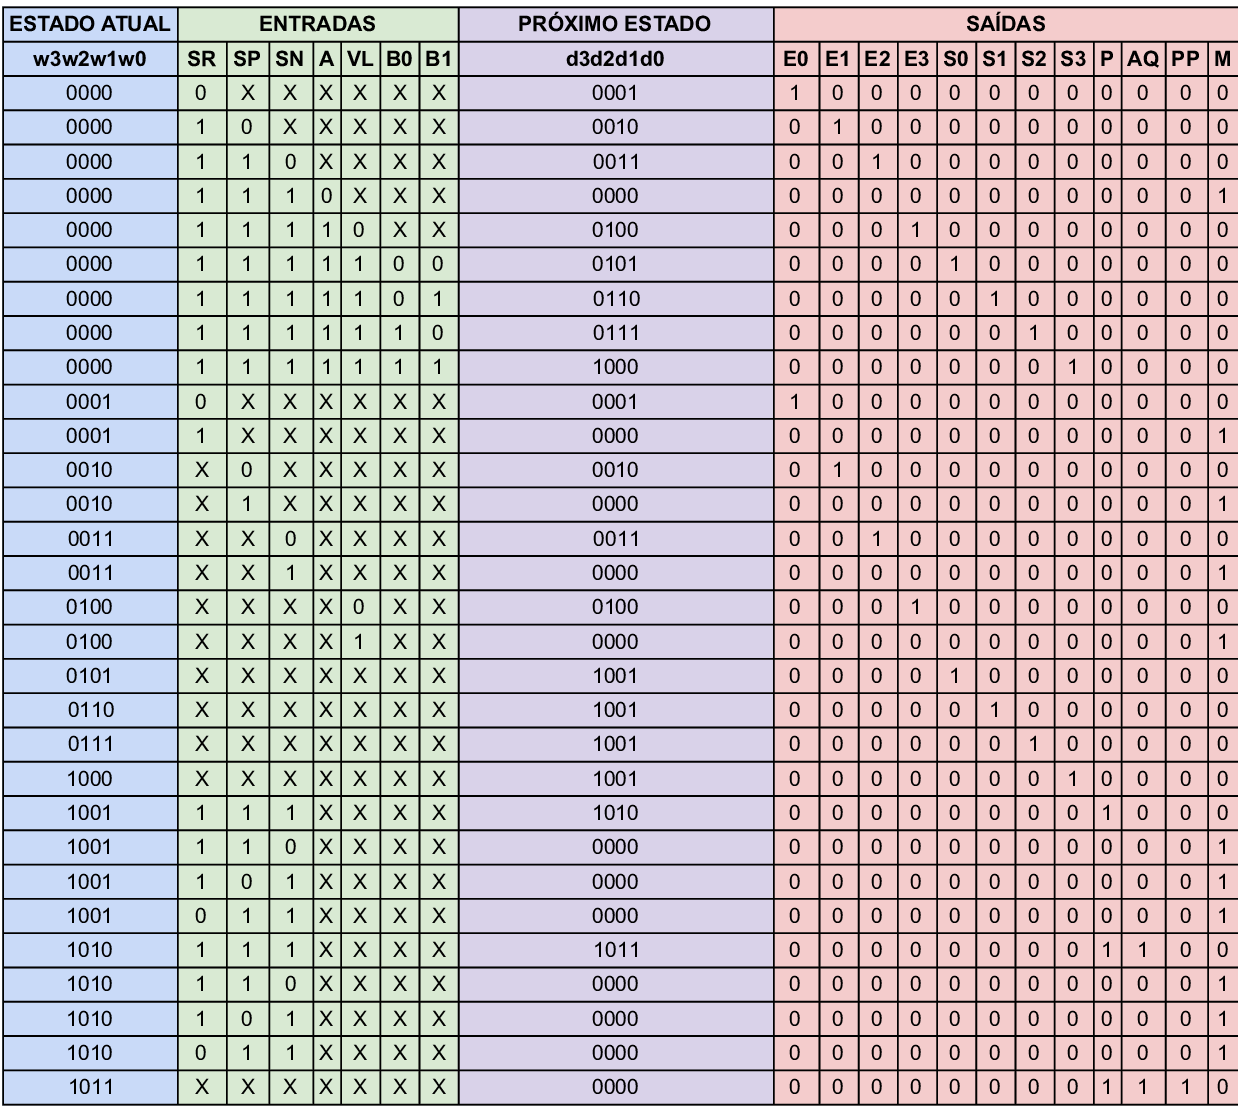
\includegraphics[width=1\textwidth]{imagens/tabelaDeExcitacao.png}
    \caption{Tabela das equações de excitação}
    \label{fig:tabelaExcitacao}
\end{figure}


O flip-flop 3 (D3) tem a seguinte expressão de saída: \~w3.\~w2.\~w1.\~w0.SR.SP.SN.A.VL.B0.B1 + \~w3.w2.\~w1.w0 + \~w3.w2.w1.\~w0 + \~w3.w2.w1.w0 + w3.\~w2.\~w1.\~w0 + w3.\~w2.\~w1.w0.SR.SN.SP + w3.\~w2.w1.\~w0.SR.SN.SP

O flip-flop 2 (D2) tem a seguinte expressão de saída: \~w3.\~w2.\~w1.\~w0.SR.SP.SN.A.\~VL + \~w3.\~w2.\~w1.\~w0.SR.SP.SN.A.VL.\~B0.\~B1 + \~w3.\~w2.\~w1.\~w0.SR.SP.SN.A.VL.\~B0.B1 + \~w3.\~w2.\~w1.\~w0.SR.\\SP.SN.A.VL.B0.\~B1 + \~w3.w2.\~w1.\~w0.\~VL

O flip-flop 1 (D1) tem a seguinte expressão de saída: \~w3.\~w2.\~w1.\~w0.SR.\~SP + \~w3.\~w2.\~w1.\~w0.SR.\\SP.\~SN + \~w3.\~w2.\~w1.\~w0.SR.SP.SN.A.VL.\~B0.B1 + \~w3.\~w2.\~w1.\~w0.SR.SP.SN.A.VL.B0.\~B1 + \~w3.\~w2.w1.\\ \~w0.\~SP + \~w3.\~w2.w1.w0.\~SN + w3.\~w2.\~w1.w0.SR.SP.SN + w3.\~w2.w1.\~w0.SR.SP.SN

O flip-flop 0 (D0) tem a seguinte expressão de saída: \~w3.\~w2.\~w1.\~w0.\~SR + \~w3.\~w2.\~w1.\~w0.SR.SP.\\ \~SN + \~w3.\~w2.\~w1.\~w0.SR.SP.SN.A.VL.\~B0.\~B1 + \~w3.\~w2.\~w1.\~w0.SR.SP.SN.A.VL.B0.\~B1 + \~w3.\~w2.\~w1.w0.\\ \~SR + \~w3.\~w2.w1.w0.\~SN +w3.\~w2.w1.\~w0.SR.SP.SN + \~w3.w2.\~w1.w0 + \~w3.w2.w1.\~w0 + \~w3.w2.w1.w0 + w3.\~w2.\~w1.\~w0

Os bits "w3", "w2", "w1" e "w0" representam a saídas dos flip-flops D3, D2, D1 e D0, respectivamente, também conhecidas comumentes como "Q". O símbolo "." representa uma porta AND e o símbolo "+" representa uma porta OR.

Contudo, as expressões acima não estão simplificadas. Com a simplificação, e a fatoração de alguns termos, através da álgebra de boole, as equações ficam da seguinte forma:

O flip-flop 3 (D3): \~w2.\~w0(SR.SP.SN.(w3 + \~w1.A.VL.B0.B1) + \~w2.\~w0) + \~w3.w2.(w1 + w0)

O flip-flop 2 (D2): \~w3.\~w1.\~w0.(\~w2.SR.SP.SN.A.(\~VL + \~B0 + \~B1) + w2.\~VL)

O flip-flop 1 (D1): \~w3.\~w2.\~w1.\~w0.SR.(\~SP + \~SN + SN.A.VL.(\~B0.B1 + B0.\~B1)) + \~w3.\~w2.w1\\(\~w0.\~SP + w0.\~SN) + w3.\~w2.SR.SP.SN(\~w1.w0 + w1.\~w0)

O flip-flop 0 (D0): \~w2.\~w0(\~w3.\~w1(\~SR + SP.(\~SN + A.VL.\~B1)) + w3.w1.SR.SP.SN) + \~w3.\~w2.w0.(\~w1.\~SR + w1.\~SN)

\section{Obtenção das equações de saída}

No caso específico deste projeto, o modelo de máquina de estados escolhido é o modelo de Mealy. Nesse modelo, as saídas do sistema dependem tanto do estado atual quanto das entradas no momento da transição entre os estados. Isso significa que a geração de saída é determinada pelo estado em que a máquina se encontra e pelas entradas recebidas nesse momento, permitindo uma maior flexibilidade e adaptabilidade do sistema. Portanto, as equações de saída terão tanto os estados quanto as entradas.

A saída E0 tem a seguinte expressão: \~w3.\~w2.\~w1.\~w0.\~SR + \~w3.\~w2.\~w1.w0.\~SR		

A saída E1 tem a seguinte expressão: \~w3.\~w2.\~w1.\~w0.SR.\~SP + \~w3.\~w2.w1.\~w0.\~SP	

A saída E2 tem a seguinte expressão: \~w3.\~w2.\~w1.\~w0.SR.SP.\~SN + \~w3.\~w2.w1.w0.\~SN								

A saída E3 tem a seguinte expressão: \~w3.\~w2.\~w1.\~w0.SR.SP.SN.A.\~VL + \~w3.w2.\~w1.\~w0.\~VL	

A saída S0 tem a seguinte expressão: \~w3.\~w2.\~w1.\~w0.SR.SP.SN.A.VL.\~B0.\~B1 + \~w3.w2.\~w1.w0		

A saída S1 tem a seguinte expressão: \~w3.\~w2.\~w1.\~w0.SR.SP.SN.A.VL.\~B0.B1 + \~w3.w2.w1.\~w0								
A saída S2 tem a seguinte expressão: \~w3.\~w2.\~w1.\~w0.SR.SP.SN.A.VL.B0.\~B1 + \~w3.w2.w1.w0								
A saída S3 tem a seguinte expressão: \~w3.\~w2.\~w1.\~w0.SR.SP.SN.A.VL.B0.B1 + w3.\~w2.\~w1.\~w0	

A saída P tem a seguinte expressão:	\~w3.w2.\~w1.w0 + \~w3.w2.w1.\~w0 + \~w3.w2.w1.w0 + w3.\~w2.\~w1.\~w0 + w3.\~w2.\~w1.w0.SR.SP.SN + w3.\~w2.w1.\~w0.SR.SP.SN + w3.\~w2.w1.w0

A saída AQ tem a seguinte expressão: w3.\~w2.\~w1.w0.SR.SP.SN + w3.\~w2.w1.w0 + w3.\~w2.w1.\\ \~w0.SR.SP.SN		

A saída PP tem a seguinte expressão: w3.\~w2.w1.\~w0.SR.SP.SN + w3.\~w2.w1.w0

A saída M tem a seguinte expressão:	\~w3.\~w2.\~w1.\~w0.SR.SP.SN.\~A + \~w3.\~w2.\~w1.w0.SR + \~w3.\~w2.w1.\~w0.SP + \~w3.\~w2.w1.w0.SN + \~w3.w2.\~w1.\~w0.VL + w3.\~w2.\~w1.w0.SR.SP.\~SN + w3.\~w2.\~w1.w0.\\SR.\~SP.SN + w3.\~w2.\~w1.w0.\~SR.SP.SN + w3.\~w2.w1.\~w0.SR.SP.\~SN + w3.\~w2.w1.\~w0.SR.\~SP.SN + w3.\~w2.w1.\~w0.\~SR.SP.SN + w3.\~w2.w1.w0			

Após a simplificação e fatoração de alguns termos utilizando a algebra de boole, as equações das saídas ficaram da seguinte forma:

Saída E0: \~w3.\~w2.\~w1.\~SR

Saída E1: \~w3.\~w2.\~w0.\~SP(SR + w1)

Saída E2: \~w3.\~w2.\~SN(\~w1.\~w0.SR.SP + w1.w0)

Saída E3: \~w3.\~w1.\~w0.\~VL(SR.SP.SN.A + w2)

Saída S0: \~w3.\~w1(\~w2.\~w0.SR.SP.SN.A.VL.\~B0.\~B1 + w2.w0)

Saída S1: \~w3.\~w0(\~w2.\~w1.SR.SP.SN.A.VL.\~B0.B1 + w2.w1)

Saída S2: \~w3.\~w2.\~w1.\~w0.SR.SP.SN.A.VL.B0.\~B1 + \~w3.w2.w1.w0

Saída S3: \~w2.\~w1.\~w0(SR.SP.SN.A.VL.B0.B1 + w3)

Saída P: \~w3.w2.(\~w1.w0 + w1) + w3.\~w2.(SR.SP.SN.(\~w1.w0. + w1.\~w0) + w1.w0 + \~w1.\~w0)

Saída AQ: w3.\~w2.SR.SP.SN.(\~w1.w0. + w1.\~w0) + w3.\~w2.w1.w0 

Saída PP: w3.\~w2.w1.(SR.SP.SN + w0)

Saída M: \~w3.\~w2.\~w1.SR(SP.SN.\~A + w0) + \~w3.\~w2.w1.(\~w0.SP + w0.SN) + \~w3.w2.\~w1.\~w0.VL + w3.\~w2.\~w1.w0.(SR.SP.\~SN + SR.\~SP.SN + \~SR.SP.SN) + w3.\~w2.w1.\~w0.(SR.SP.\~SN + SR.\~SP.SN + \~SR.SP.SN) + w3.\~w2.w1.w0

\section{Desenho do circuito}

O circuito foi desenhado utilizando o software Logisim, que é um simulador lógico que permite o desenho de circuitos. Com ele, foi possível desenhar as portas lógicas e as relações de entradas e saídas. Além disso, ele permite efetuar a simulação e teste do circuito. A Figura 5 apresenta todo o circuito da MEF desenvolvida.

\begin{figure}[!h]
    \centering
    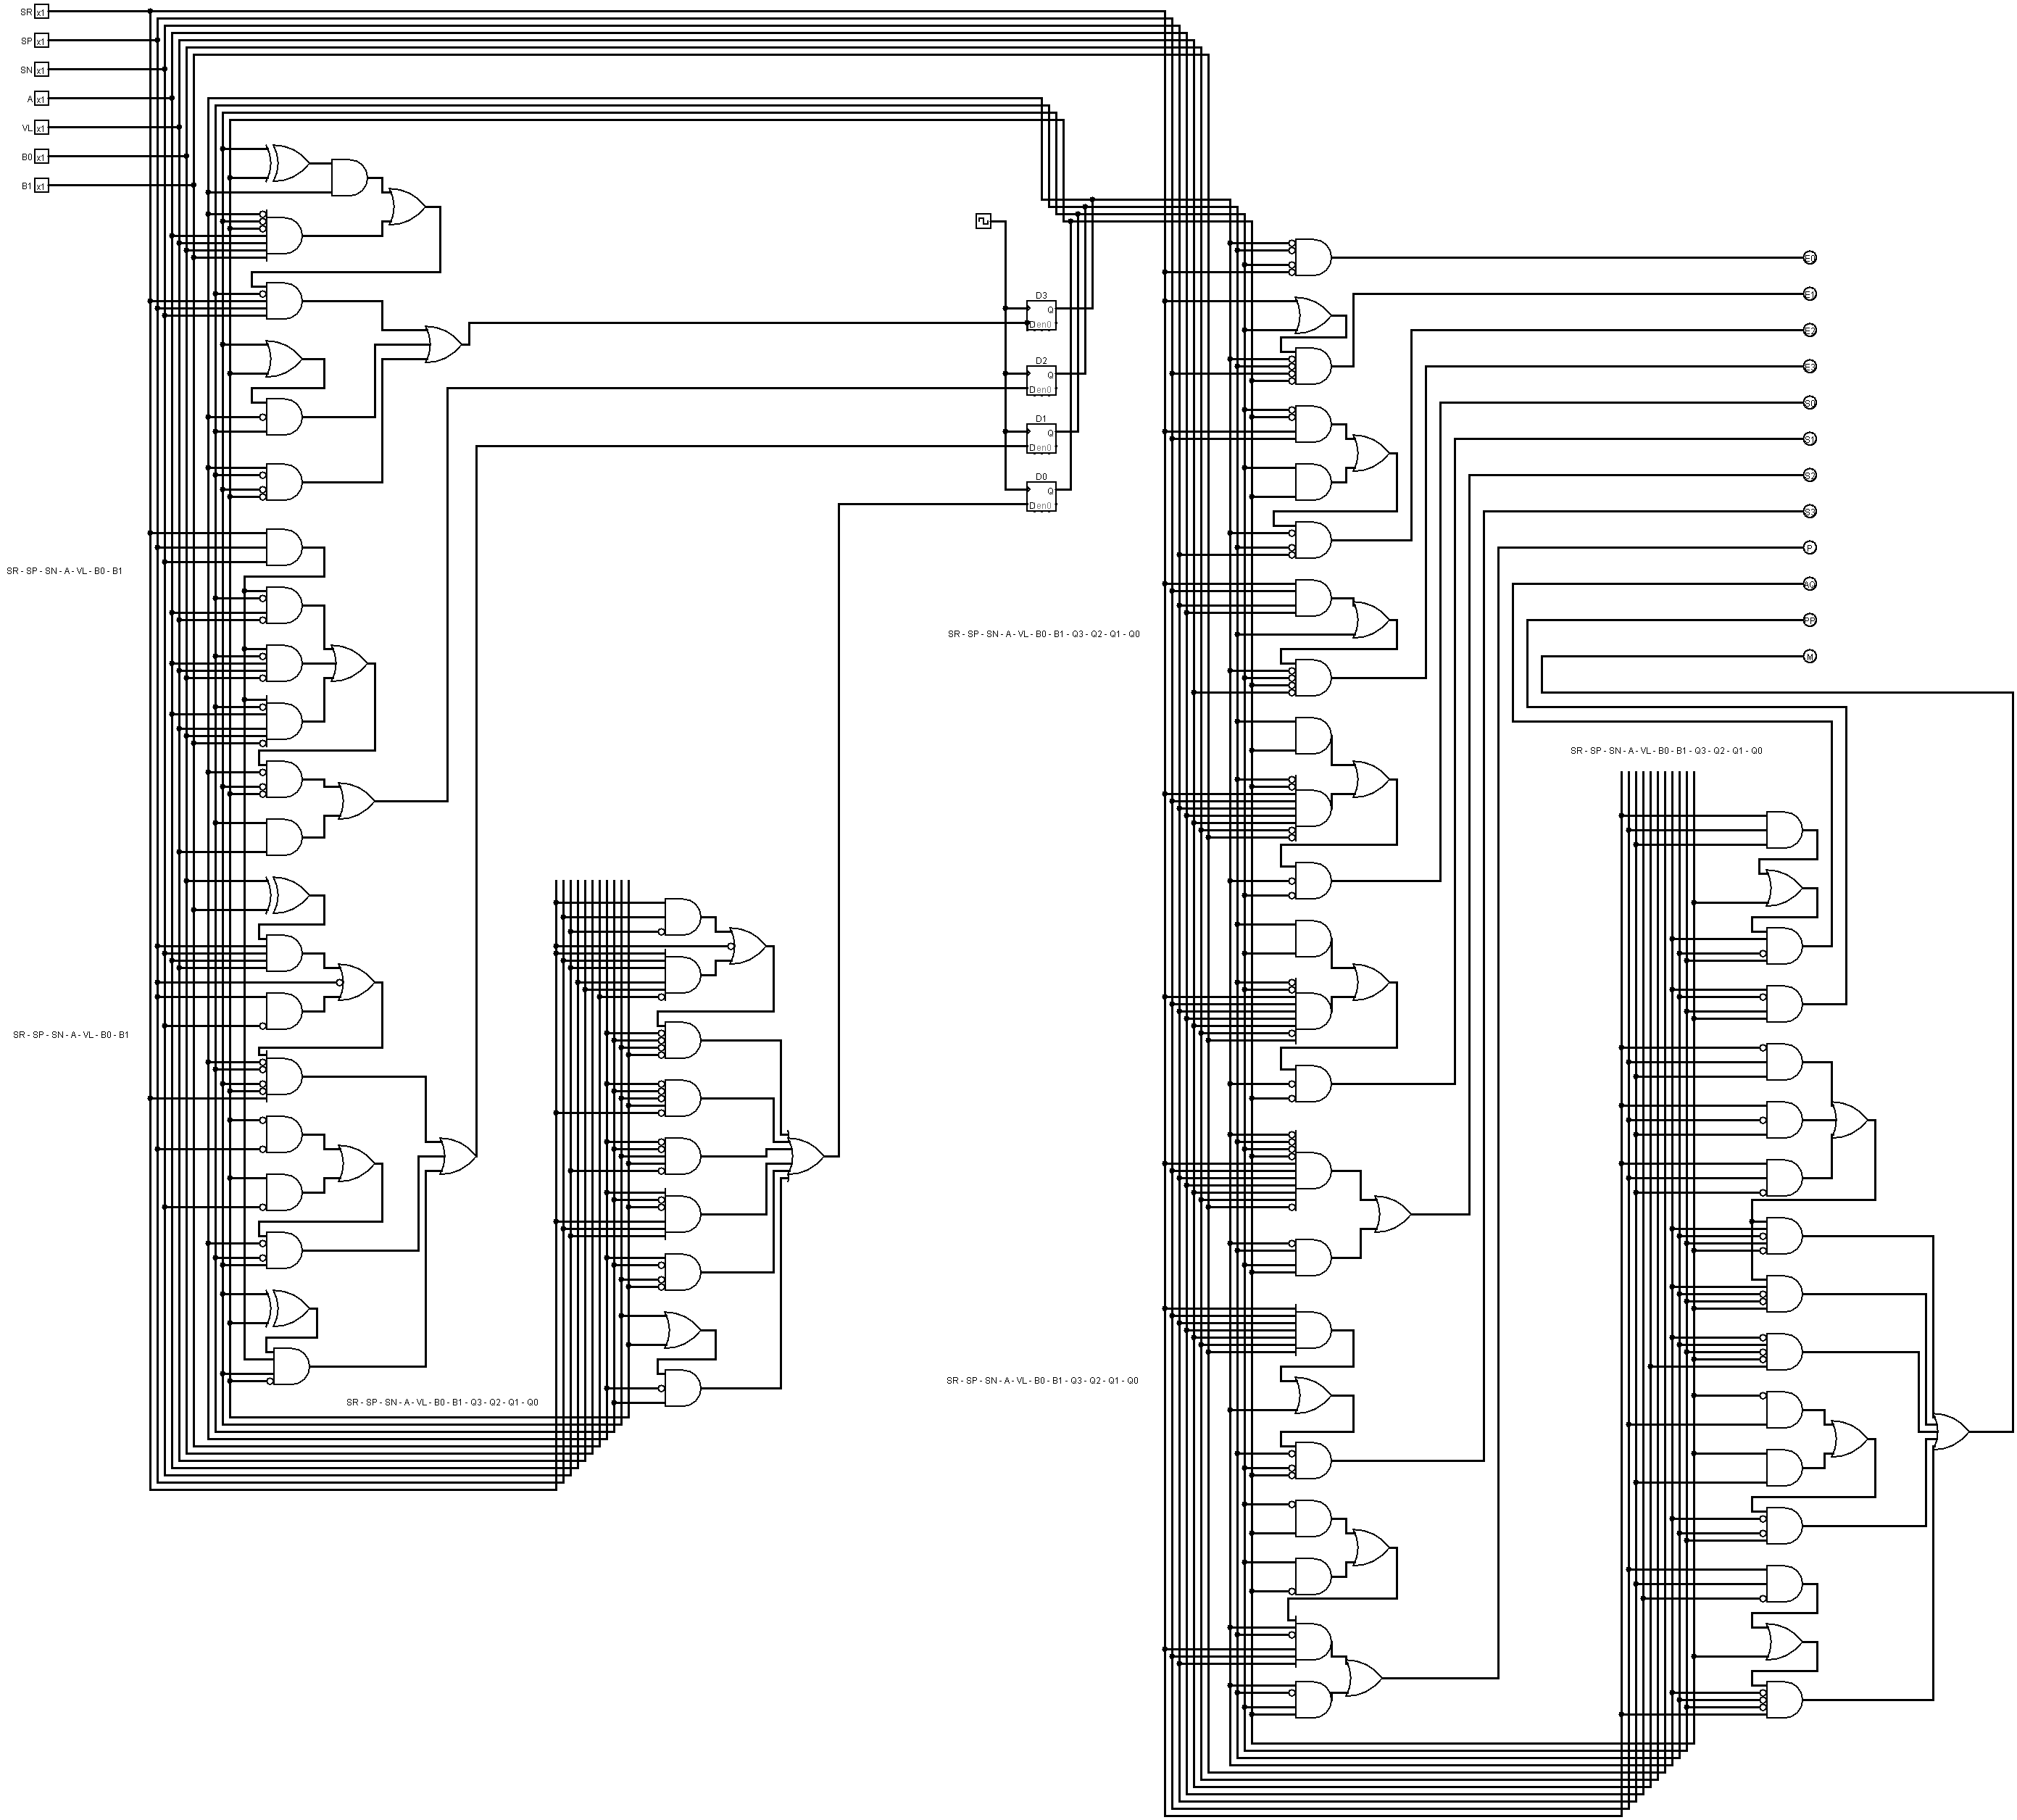
\includegraphics[width=1\textwidth]{imagens/DesenhoCircuito.png}
    \caption{Desenho do circuito lógico}
    \label{fig:desenhoCircuito}
\end{figure}

\section{Teste e simulação}

Algumas simulações utilizando o software do Logisim foram utilizadas para realizar os testes de funcionalidades da máquina de estados. As entradas foram movidas para próximo das saídas para que fosse melhor visualizado o comportamento das saídas de acordo com as entradas.

Como é possível verificar na simulação da Figura 6, todas as entradas possuem nível lógico baixo, com isso a saída E0 é apresentada, informando que o sensor SR está recebendo nível lógico baixo.

\begin{figure}[]
    \centering
    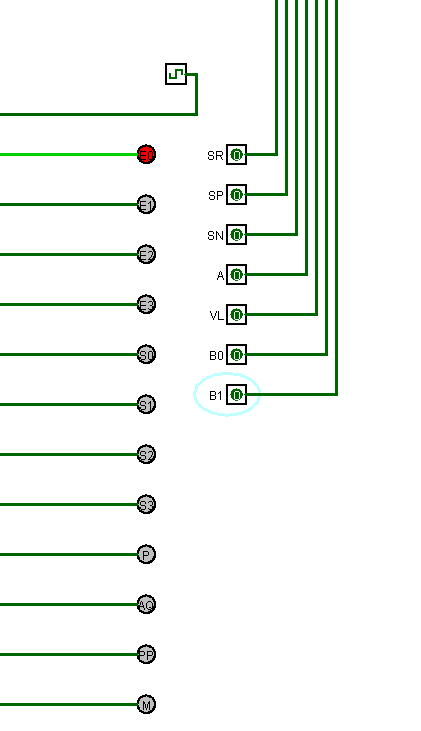
\includegraphics[width=0.3\textwidth]{imagens/simulacao1.png}
    \caption{Simulação com entradas 0000000 e saídas 1000000000000}
    \label{fig:simulacao1}
\end{figure}

Na segunda simulação (Figura 7), o sensor SR envia nível lógico alto, mas as outras entradas continuam recebendo nível lógico baixo, o que possibilita que a saída E1 seja apresentada, informando que o sensor SP está enviando nível lógico baixo.

\begin{figure}[]
    \centering
    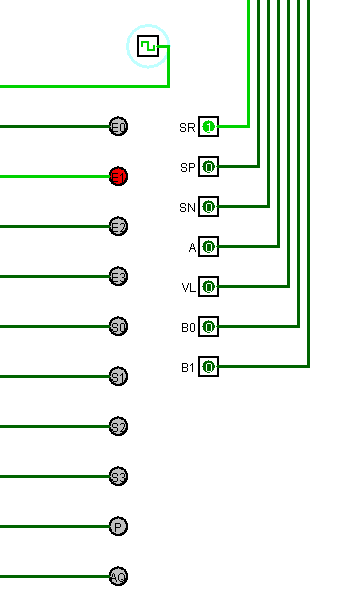
\includegraphics[width=0.3\textwidth]{imagens/simulacao2.png}
    \caption{Desenho do circuito }
    \label{fig:simulacao2}
\end{figure}

Com todos os sensores enviando nível lógico alto (Figura 8), a MEF entra em estado inicial. A saída apresentada é o modo de espera. Com isso o usuário pode modificar as entradas para acionar o preparo.

\begin{figure}[]
    \centering
    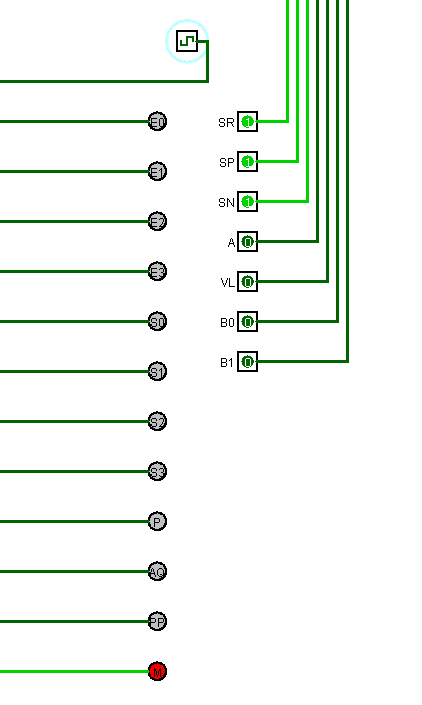
\includegraphics[width=0.35\textwidth]{imagens/simulacao3.png}
    \caption{ do circuito lógico}
    \label{fig:simulacao3}
\end{figure}

Por fim, na Figura 9 é possível verificar, após acionamento com a entrada "A", com todos os sensores em nível lógico alto, junto com o VL, e a escolha de bebida B0=0 e B1=1, a saída S1 é apresentada, informando o tipo de bebida selecionado.

\begin{figure}[]
    \centering
    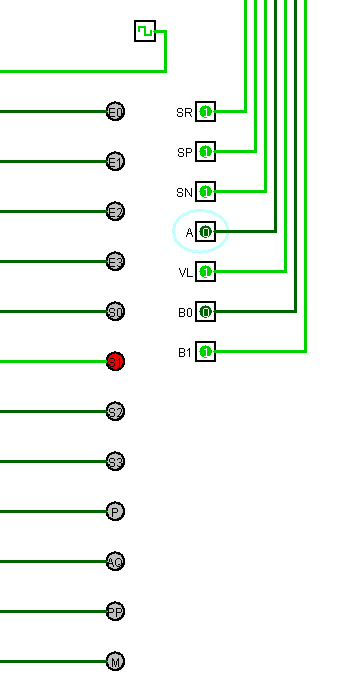
\includegraphics[width=0.3\textwidth]{imagens/simulacao4.png}
    \caption{Desenho d lógico}
    \label{fig:simulacao4}
\end{figure}

Outras simulações foram feitas, mas devido a quantidade de possibilidades de testes a serem feitos, não cabe a inserção neste relatório técnico.

\section{Descrição do código}
O código gerado contém a descrição do módulo chamado "MainCoffeeMachine". Esse módulo é parte principal da lógica da máquina de café e desempenha um papel crucial na coordenação das funcionalidades da máquina. O módulo possui várias entradas e saídas, incluindo sinais de controle como CLK, SR, SP, SN, A, V0, V1, B0 e B1, bem como sinais de saída para o display de sete segmentos (a, b, c, d, e, f, g, h, dig1, dig2, dig3, dig4) e para os LEDs (P, AQ, PP). O sinal de reticências ("...") na imagem representa continuação do código seguindo a mesma lógica do trecho posterior.

\begin{figure}[!h]
    \centering
    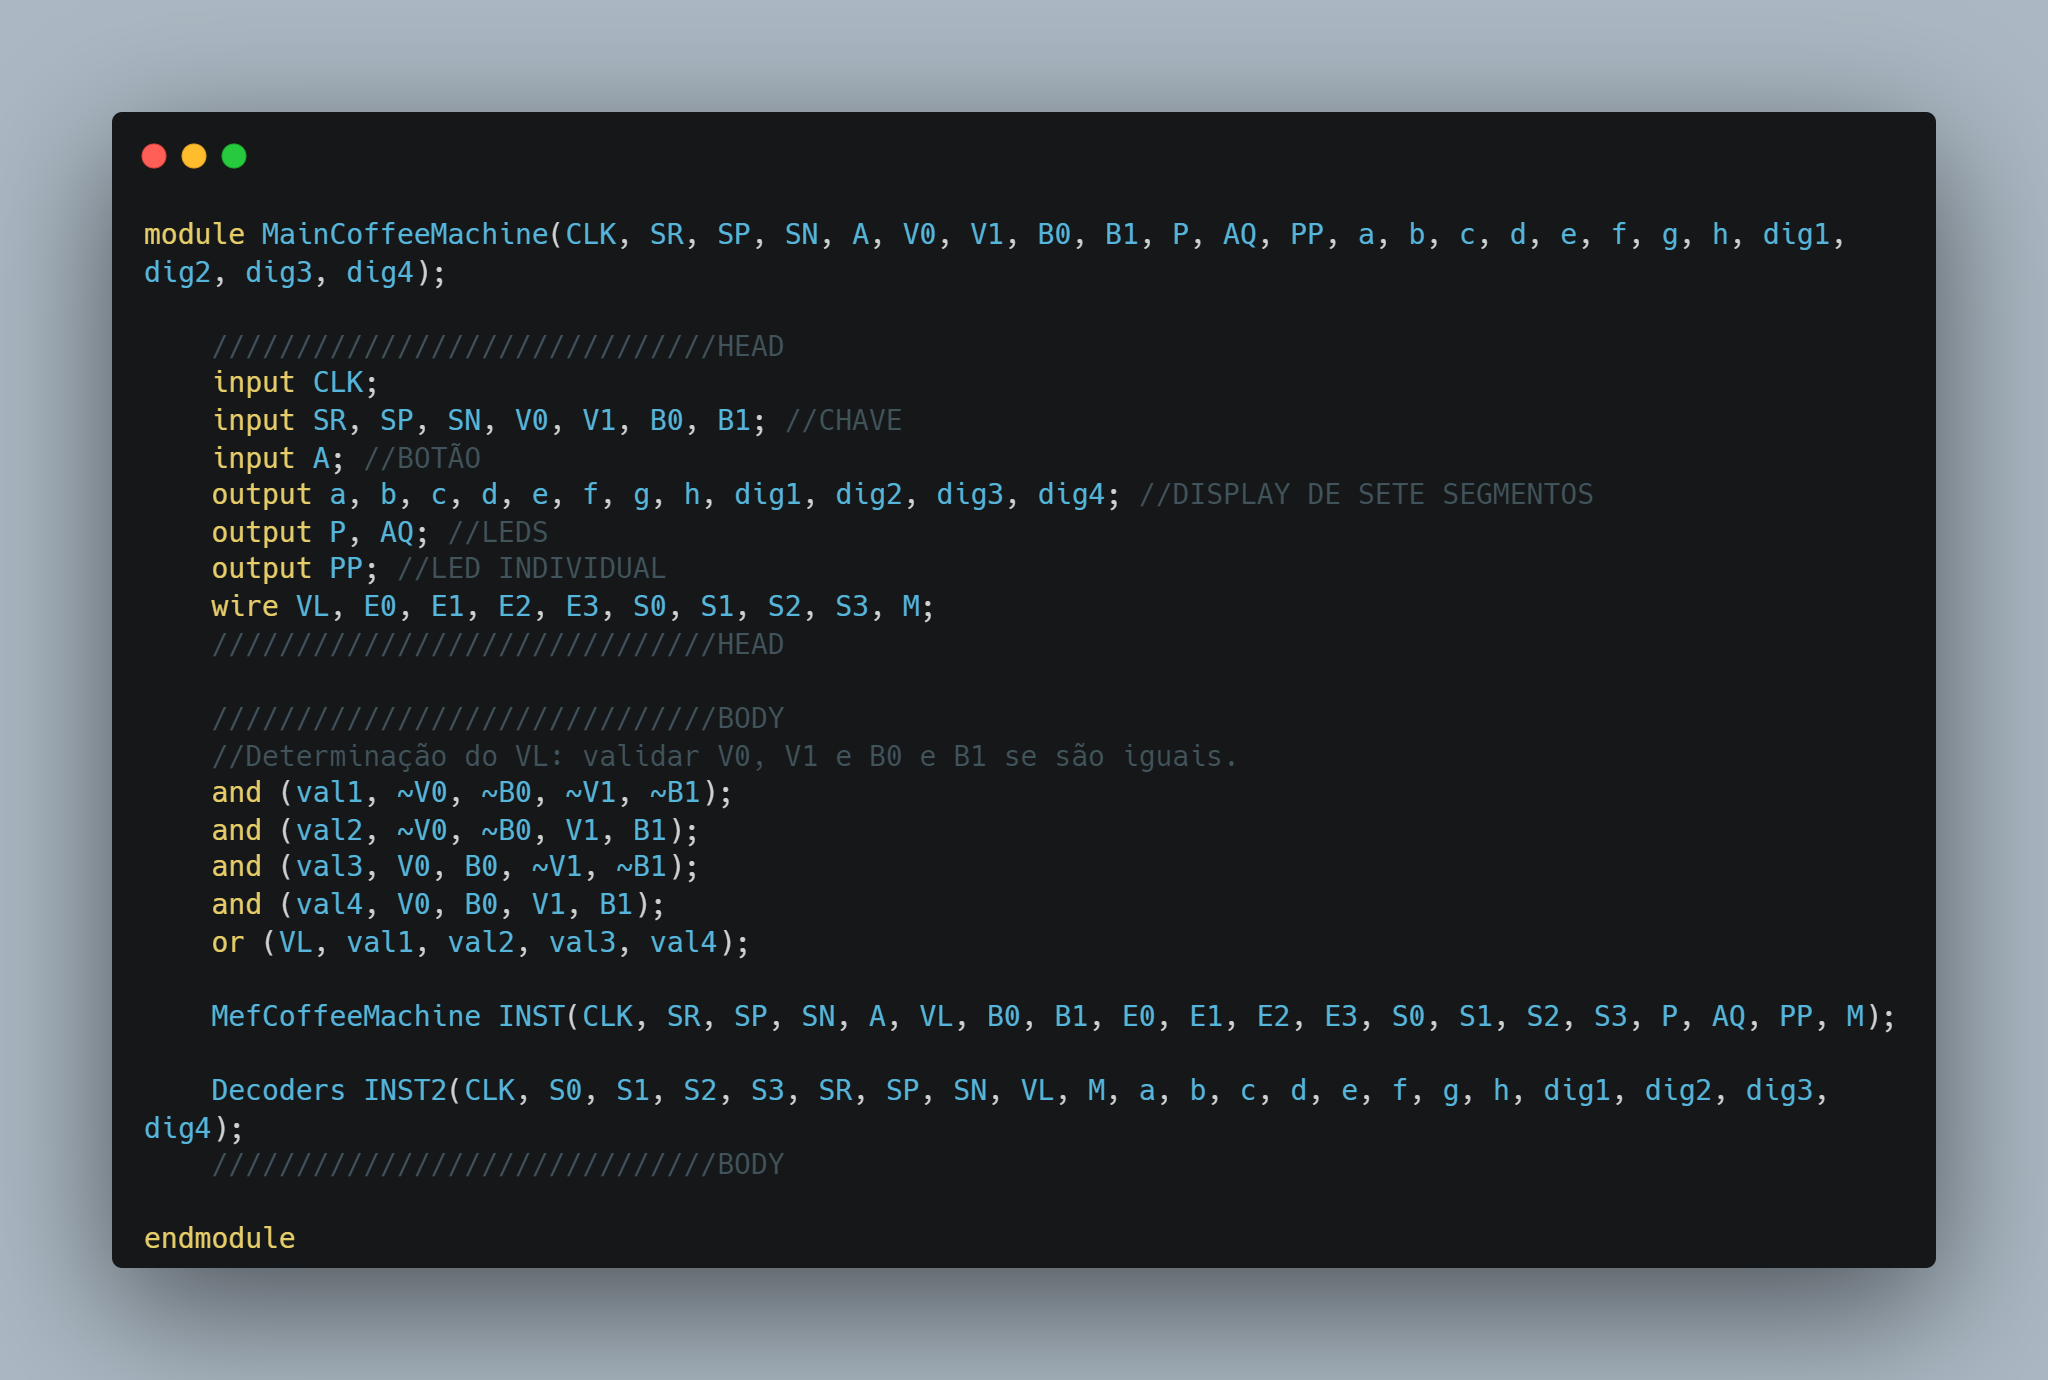
\includegraphics[width=1\textwidth]{imagens/carbon_main.png}
    \caption{Módulo principal do código importando os módulos da MEF e dos decodificadores}
    \label{fig:carbon_main}
\end{figure}

Dentro do módulo, são declarados sinais de fio que serão utilizados posteriormente, como VL, E0, E1, E2, E3, S0, S1, S2, S3 e M. Esses sinais são usados para conectar os diferentes componentes do sistema e garantir o correto funcionamento da máquina de café.

Uma parte importante do código é a determinação do valor de VL. Isso é feito através do uso de portas lógicas, como AND e OR, que verificam as combinações das entradas V0, V1, B0 e B1. O objetivo é determinar se essas entradas são iguais ou diferentes, e o resultado é atribuído ao sinal VL.

Além disso, o módulo "MainCoffeeMachine" instancia dois outros módulos: "MefCoffeeMachine" e "Decoders". O primeiro é instanciado como "INST" e recebe diversas entradas e saídas, incluindo os sinais de controle, VL, B0, B1, e os sinais de saída P, AQ, PP e M. O segundo é instanciado como "INST2" e também recebe várias entradas e saídas, como os sinais de controle e os sinais de saída para o display de sete segmentos.

Esses módulos adicionais desempenham funções específicas dentro do sistema da máquina de café. O "MefCoffeeMachine" implementa a lógica de controle principal da máquina, enquanto o "Decoders" é responsável por converter os sinais de controle em sinais adequados para o display de sete segmentos, permitindo a exibição das informações através das interfaces.

O módulo "MefCoffeeMachine" é responsável por implementar a lógica de controle da máquina, permitindo que ela funcione corretamente. Dentro do módulo, são declarados sinais de fio que serão utilizados posteriormente, como Q3, Q2, Q1, Q0 e uma série de sinais w1 a w41 e s1 a s56. É utilizado quatro flip-flops (FFD) para armazenar o estado atual da máquina de café. Os sinais w1 a w41 são usados para codificar as equações de excitação dos estados e determinar o próximo estado com base nas entradas e no estado atual.

\begin{figure}[!h]
    \centering
    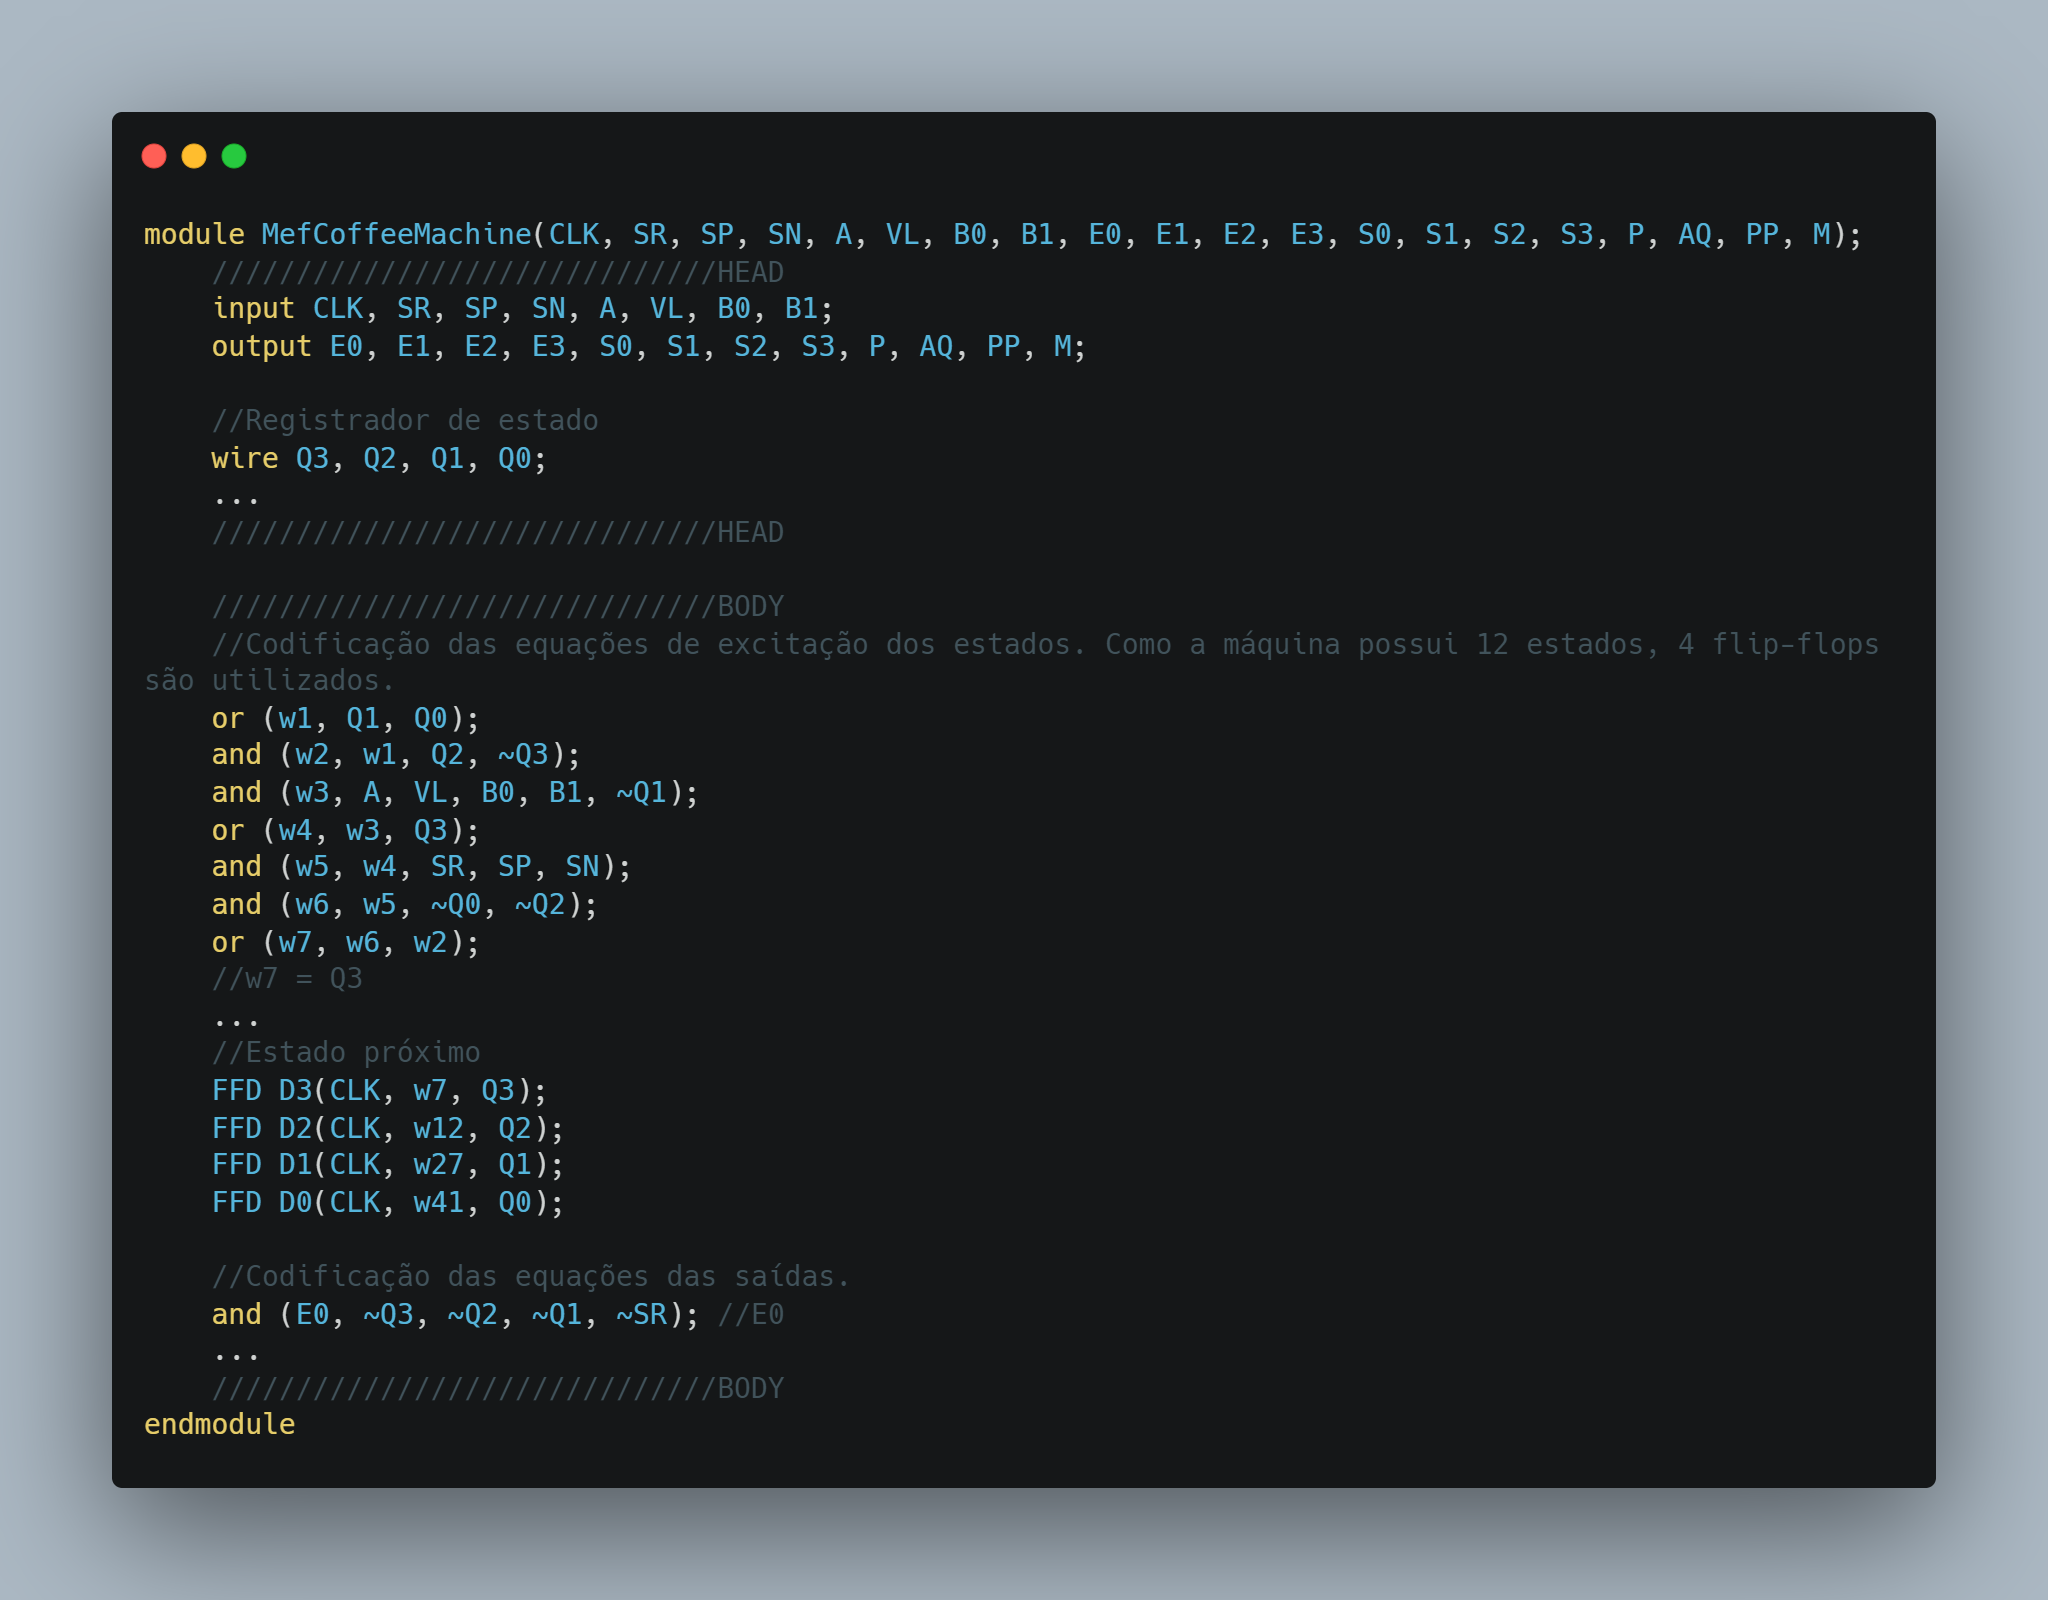
\includegraphics[width=1\textwidth]{imagens/carbon_mef.png}
    \caption{Módulo de implementação da Máquina de Estados Finitos}
    \label{fig:carbon_mef}
\end{figure}

Em seguida, são codificadas as equações das saídas da máquina. Os sinais E0, E1, E2, E3, S0, S1, S2 e S3 representam as saídas específicas da máquina, que serão enviadas para os decodificadores como análise das interfaces do display de sete segmentos. Por fim, P, AQ e PP representam a pressurização, aquecimento e informação de bebida disponível para retirada, respectivamente. Esses sinais são enviados para o bloco principal.

O módulo MEF também instancia o módulo de delay, dando 2 segundos para as saídas do pressurizador e aquecedor serem disponibilizadas. Como, em sessão, foi permitido a utilização de um código comportamental, o Delay foi importado do módulo DelayedOutput. Como esse bloco de código utiliza bastante recurso, foi apenas utilizado nas saídas do pressurizador e aquecedor, completando os requisitos solicitados no problema. 

O módulo Decoders é responsável por enviar os sinais de acordo com a interface selecionada pela máquina de estados. O módulo possui uma série de decodificadores, que são comumente utilizados para exibir dígitos em displays de 7 segmentos, em que cada segmento pode ser ativado ou desativado para formar diferentes caracteres numéricos ou alfanuméricos. Os seguintes códigos alfanuméricos a serem exibidos no display de sete segmentos estão representados pelos seguintes sinais:

\begin{itemize}
    \item "CE01": escolha do S0;
    \item "CL02": escolha do S1;
    \item "CC05": escolha do S2;
    \item "CP10": escolha do S3;
    \item "ERSR": erro do sensor SR;
    \item "ERSP": erro do sensor SP;
    \item "ERSN": erro do sensor SN;
    \item "ERDI": erro de validação do valor/dinheiro;
    \item "....": modo de espera.
\end{itemize}

\begin{figure}[!h]
    \centering
    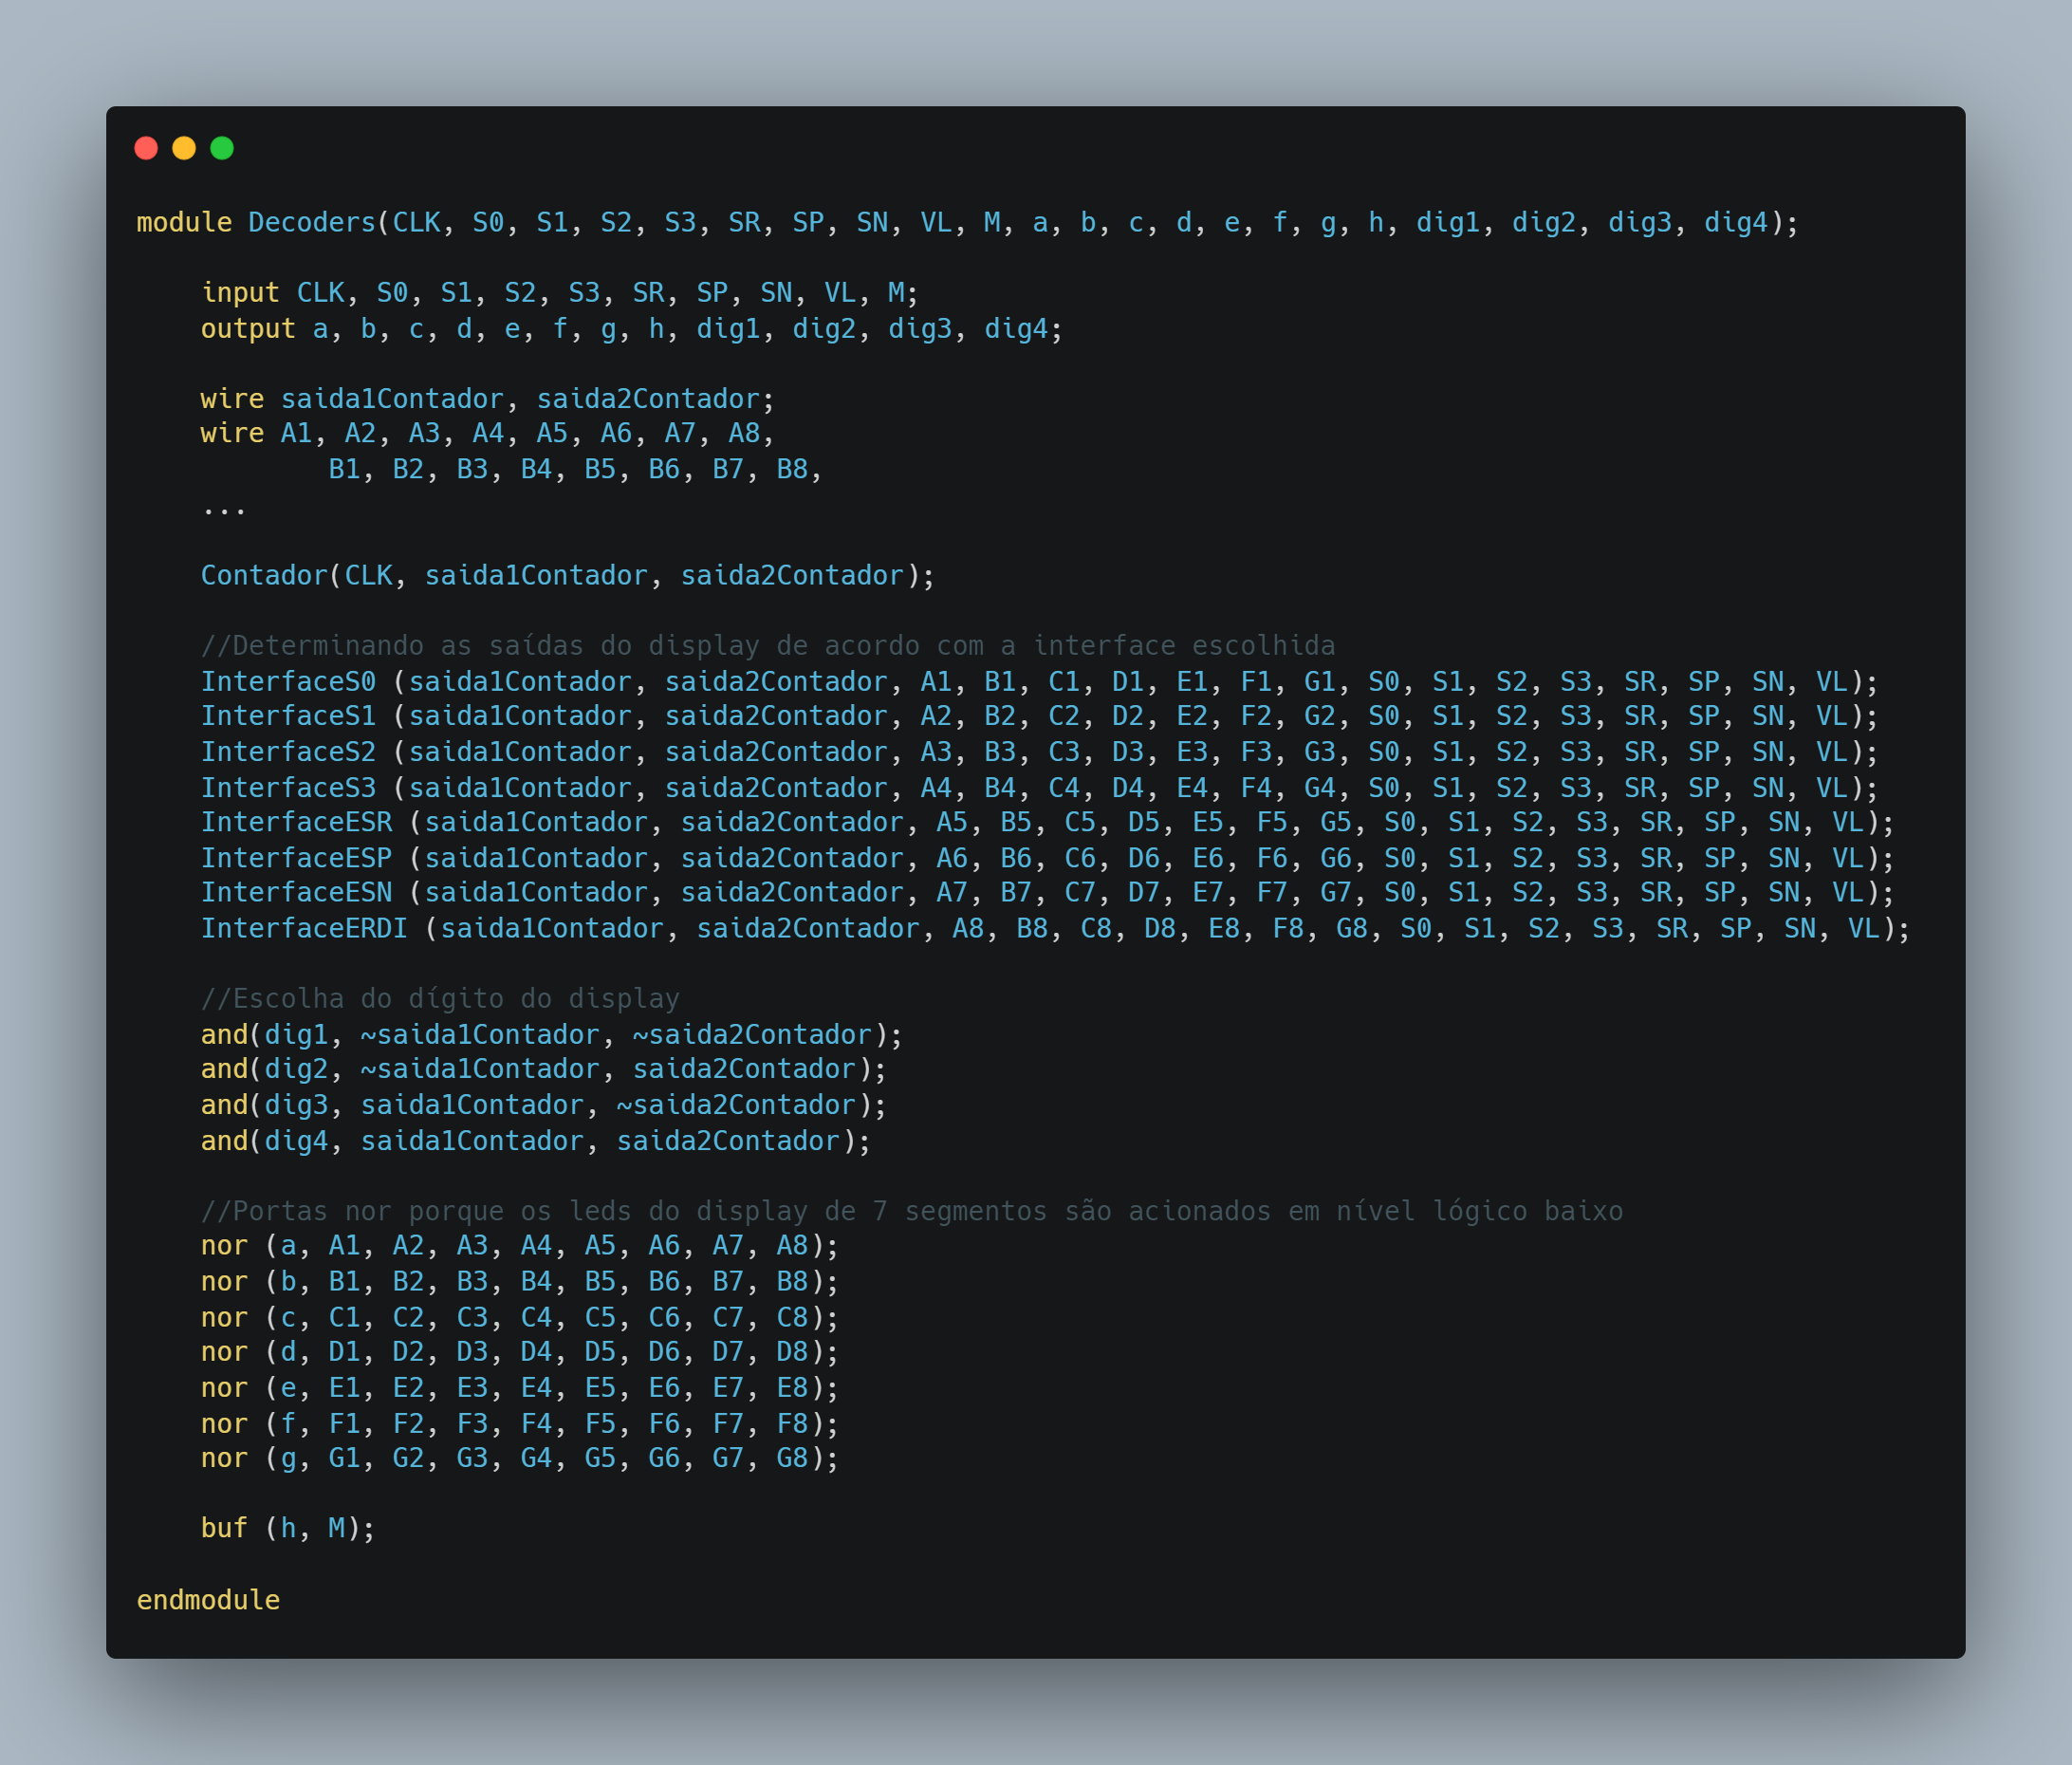
\includegraphics[width=1\textwidth]{imagens/carbon_decoders.png}
    \caption{Módulo de implementação dos decodificadores das interfaces de saída}
    \label{fig:carbon_decoders}
\end{figure}

O módulo "Decoders" possui diversas entradas e saídas que são utilizadas para controlar e exibir os dígitos no display. Para implementar a funcionalidade do decodificador de 7 segmentos, o módulo faz uso de outros módulos e interfaces. O módulo Contador é utilizado para gerar dois sinais de saída (saida1Contador e saida2Contador), que determinam o dígito atual a ser exibido no display. Esses sinais são utilizados como entrada para as interfaces correspondentes (InterfaceS0, InterfaceS1, InterfaceS2, InterfaceS3, InterfaceESR, InterfaceESP, InterfaceESN, InterfaceERDI), que recebem também os sinais de controle. Cada interface é responsável por gerar os sinais de saída correspondentes aos segmentos do display de 7 segmentos, dependendo das combinações específicas dos sinais de controle.

Além disso, o código implementa a lógica de seleção do dígito atual a ser exibido. Por meio de portas lógicas and, os sinais saida1Contador e saida2Contador são combinados com sinais complementares para ativar apenas um dígito por vez. Os sinais resultantes (dig1, dig2, dig3, dig4) são utilizados para selecionar o dígito apropriado no display.

Por fim, as portas nor são utilizadas para combinar os sinais dos segmentos individuais (A1 a A8, B1 a B8, etc.) em um único sinal para cada segmento do display (a, b, c, d, e, f, g). Esses sinais combinados representam os segmentos ativados ou desativados para exibir o dígito atual no display de 7 segmentos.

O sinal h é conectado diretamente à entrada M por meio de um buffer (buf) para exibir um ponto decimal, representando o modo de espera no display.

\section{Recursos físicos}

Sem o código comportamental do Delay, a implementação consumiu os seguintes recursos:

\begin{figure}[!h]
    \centering
    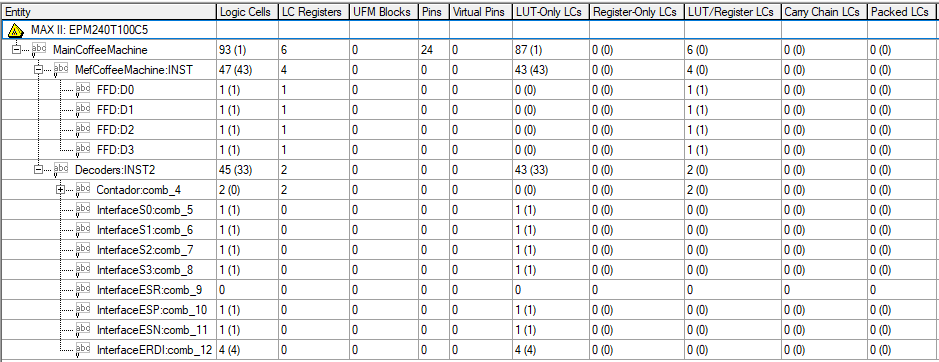
\includegraphics[width=1\textwidth]{imagens/hierarchy_info.png}
    \caption{Tabela de consumo de recursos físicos do código}
    \label{fig:hierarchy_info}
\end{figure}

\chapter{RESULTADOS}
Por fim, a MEF realizada apresentou resultados positivos em todos os testes realizados. Entretanto, isso não resume todo o projeto. No início houve dificuldade na escolha do tipo de máquina, em qual seria mais ideal para a implementação do problema proposto. Não obstante, com reforço no referencial teórico e na percepeção da necessidade das saídas em lidarem com as entradas, foi definido o tipo de Mealy. Correções foram feitas em todo o processo e isso fez com que a construção tenha sido contínnua, o que definiu um resultado mais embasado e fortificado em todos os seus processos. Com isso, o projeto está pronto para ser aplicado fisicamente com todas as adaptações necessárias.



\postextual
\endgroup

% ----------------------------------------------------------
% Referências bibliográficas
% ----------------------------------------------------------
\bibliography{bibliografia}

\end{document}
